\documentclass[12pt,a4paper]{article}
\usepackage[UTF8]{ctex}
\usepackage{amsmath,amssymb}
\usepackage{xcolor}
\usepackage{hyperref}
\usepackage{geometry}
\usepackage{graphicx}
\geometry{margin=2.5cm}

\title{Noise Model / 噪声模型}
\author{QuoNic}
\date{}

\begin{document}
\maketitle

\begin{center}
\textbf{Noise / 噪声} | 难度：中级 | 预计时间：15 分钟
\end{center}

\tableofcontents
\newpage

\section{为什么需要？}

噪声模型用于模拟量子硬件中的噪声。

\subsection{经典局限}
\begin{itemize}
  \item 经典计算没有量子噪声
  \item 量子噪声会破坏计算结果
\end{itemize}

\subsection{量子优势}
\begin{itemize}
  \item 噪声模型可以模拟真实量子硬件
  \item 用于测试量子算法的鲁棒性
  \item 指导量子硬件设计
\end{itemize}

\subsection{实际应用}
\begin{itemize}
  \item 量子硬件仿真
  \item 量子算法测试
  \item 量子硬件设计
\end{itemize}

\section{快速上手}

\begin{verbatim}
from quonic.noise import noise_model

# 创建噪声模型
model = noise_model(error_rate=0.01, noise_type='depolarizing')
print(f'Noise model: {model}')
\end{verbatim}

\textbf{预期输出}：
\begin{verbatim}
Noise model: depolarizing(0.01)
\end{verbatim}

\section{原理详解}

\subsection{电路图}

\begin{center}
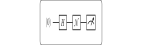
\includegraphics[width=0.6\textwidth]{../../images/noise_model_circuit.svg}
\end{center}

\subsection{数学推导}

噪声模型：
\begin{equation}
\mathcal{E}(\rho) = (1-p)\rho + \frac{p}{3}(X\rho X + Y\rho Y + Z\rho Z)
\end{equation}

\subsection{几何解释}

噪声模型在 Bloch 球上使量子态退相干。退极化噪声使量子态趋向混合态。

\section{代码详解}

\begin{verbatim}
from quonic.noise import noise_model

# noise_model(error_rate, noise_type)
# error_rate: 错误概率
# noise_type: 噪声类型 ('depolarizing', 'bit_flip', 'phase_flip')

model = noise_model(
    error_rate=0.01,
    noise_type='depolarizing'
)

# model: 噪声模型
# model.apply(circuit): 应用噪声
print(f'Noise model: {model}')
\end{verbatim}

\section{进阶用法}

\subsection{场景 1：不同噪声类型}

\begin{verbatim}
from quonic.noise import noise_model

# 不同噪声类型
m1 = noise_model(error_rate=0.01, noise_type='depolarizing')
m2 = noise_model(error_rate=0.01, noise_type='bit_flip')
m3 = noise_model(error_rate=0.01, noise_type='phase_flip')
\end{verbatim}

\subsection{场景 2：不同错误率}

\begin{verbatim}
from quonic.noise import noise_model

# 不同错误率
for p in [0.001, 0.01, 0.1]:
    model = noise_model(error_rate=p)
    print(f'p={p}: {model}')
\end{verbatim}

\section{适用场景}

\subsection{量子硬件仿真}

噪声模型用于模拟真实量子硬件的噪声。这有助于测试量子算法的鲁棒性。

\subsection{量子算法测试}

噪声模型用于测试量子算法在噪声环境下的性能。这有助于优化量子算法。

\section{常见问题}

\subsection{噪声模型有哪些类型？}

常见的噪声类型包括：退极化噪声、比特翻转噪声、相位翻转噪声、退相干噪声等。

\subsection{噪声模型的精度如何？}

噪声模型的精度取决于噪声参数的选择。更精确的噪声模型需要更多的参数。

\section{学习路径}

\subsection{前置知识}
\begin{itemize}
  \item 量子噪声
  \item 量子测量
  \item 量子门
\end{itemize}

\subsection{继续学习}
\begin{itemize}
  \item 误差缓解
  \item 量子纠错
  \item 量子硬件
\end{itemize}

\section{完整示例代码}

\subsection{示例 1：基本噪声模型}

\begin{verbatim}
from quonic.noise import noise_model

model = noise_model(error_rate=0.01, noise_type='depolarizing')
print(f'Noise model: {model}')
\end{verbatim}

\section{下载}

\begin{itemize}
  \item [noise\_model.py](https://github.com/ChrisLee0721/QuoNic/blob/main/examples/noise_model/noise_model.py)
\end{itemize}

\end{document}
